\subsection{Data Analysis}

A total of 3489 stories will be analyzed in two parts: a topic model using Latent Dirichlet Allocation (LDA) and a sentiment analysis using the VADER sentiment analysis tool. The topic model will be used to identify the most common topics in the stories and the sentiment analysis will be used to identify the sentiment of the stories.

\subsection{Topic Modelling}

As mentioned in the introduction, topic modeling is a text-mining method to identify and classify data. More specifically, topic modeling is used to identify topics in a corpus of documents and classifying a distribution of words to them. A simple example would be that a sentence containing the words "politician bill government president economic growth" could be attributed to a topic "politics". We can also see that the words "economic" and "growth" could also be attributed to another topic "economy". Topic modeling extrapolates this idea to a corpus of documents and identifies the most common topics in the corpus. There are many methods to perform topic modeling, all with their own use cases, as well as advantages and disadvantages.~\cite{abdelrazek2022topic} For example, Non-negative Matrix Factorization (NMF) and BERTopic are examples of topic models that are more suited for tweets than other topic models like Latent Dirichlet Allocation (LDA).~\cite{egger2022topic} LDA seems to be frequently used to analyze abstracts of scientific papers, which are similar in length to the stories in the dataset. This was the basis for the decision to use LDA topic modeling in this project.

\subsubsection{Latent Dirichlet Allocation (LDA)}

LDA was proposed in 2003 by Blei, Ng and Jordan. It is a generative probabilistic model that assumes that each document is a mixture of topics and that each word in the document is attributable to one of the document's topics.~\cite{NIPS2001_296472c9} The most basic assumptions are the following:

\begin{itemize}
    \item There are $K$ topics in the corpus of documents that are distributed according to a Dirichlet distribution with the hyperparameter $\alpha$.
    \item Each document is a mixture of the $K$ topics.
    \item Each word in the document is attributable to one of the $K$ topics and is distributed according to a Dirichlet distribution with the hyperparameter $\beta$.
\end{itemize}

For this paper, the LDA module of python's gensim library is used.~\cite{rehurek_lrec} The gensim LDA implementation is based on Hoffman and David's implementation. The above mentioned distributions are considered to be the prior distributions. The posterior distributions are then calculated using collapsed Gibbs sampling.

\subsubsection{Parameter Tuning}

Just like with any other machine learning model, there are parameters that play a crucial role in the accuracy of the model. These parameters are assumptions that we have to make. However, choosing the right parameters can be a complicated process.

\subsubsection*{Evaluation Metric}

Topic models should produce results that are interpretable by humans. This should be the metric that is used to evaluate the model. Obviously, it is not feasible to evaluate all models by hand. Instead, we can use metrics that are correlated with human interpretability. Examples of such metrics are the coherence score and the perplexity score. However, perplexity is not a good metric for topic models, as there are indications that it correlates negatively with human interpretability. The coherence score is a better metric, but it is not perfect either.~\cite{egger2022topic} Furthermore, there are different types of coherence scores, like the $C_v$ coherence score, the $C_{uci}$ coherence score and the $C_{npmi}$ coherence score. The $c_v$ coherence score is the most commonly used coherence score. Based on the claim that the $C_v$ score correlates highest with human ratings, it will be used in this project.~\cite{roder2015exploring} The coherence score is a value between 0 and 1, with 1 being the highest coherence score. Though high values may indicate a "too good to be true" case.  %TODO: Add source%

\subsubsection*{The Parameters}

The coherence of a produced topic model depends on the assumptions it makes. In other words, the choice of hyperparameters decides how coherent the model is, therefore it is important to choose the right parameters. The parameters to consider are list in table 2:

\begin{table}[h]
    \centering
    \begin{tabular}{cl}
        \hline
        Parameter & Description \\
        \hline
        $K$ & Number of topics \\
        $\alpha$ & The hyperparameter of the Dirichlet distribution of the topics\\
        $\beta$ & The hyperparameter of the Dirichlet distribution of the words  \\
          &  in each topic \\
        $min\_df$ & Minimum proportion of documents a word must appear in \\
        $max\_df$ & The maximum proportion of documents a word can appear in \\
\end{tabular}
    \caption{Parameters to consider when tuning the LDA model.}
    \label{tab:parameters}
\end{table}

As mentioned before, the LDA model has two hyperparameters $\alpha$ and $\beta$. In this project, $\alpha$ is a singular scalar value that is used for all topics. For example, if we have $K=3$ topics and $\alpha=0.1$, then the Dirichlet distribution for the topics would be $\textbf{Dir}(0.1, 0.1, 0.1)$. $\beta$ is as well a singular scalar value that is used for all words in the corpus. For example, if we have $V=1000$ words in the corpus and $\beta=0.1$, then the Dirichlet distribution for the words would be $\textbf{Dir}(0.1, 0.1, ..., 0.1)$ with $V$ values.

Due to the nature of Dirichlet distributions, low values of hyperparameters produce sparse distributions, while high values produce more uniform distributions. This means that low values of $\alpha$ assume that each document will be dominated by a few topics, while high values assume that each document will contain a mixture of more-or-less all topics. Similarly, low values of $\beta$ assume that each topic will be dominated by a few words, while high values assume that each topic will contain a mixture of more words.

\begin{figure}[h]
    \centering
    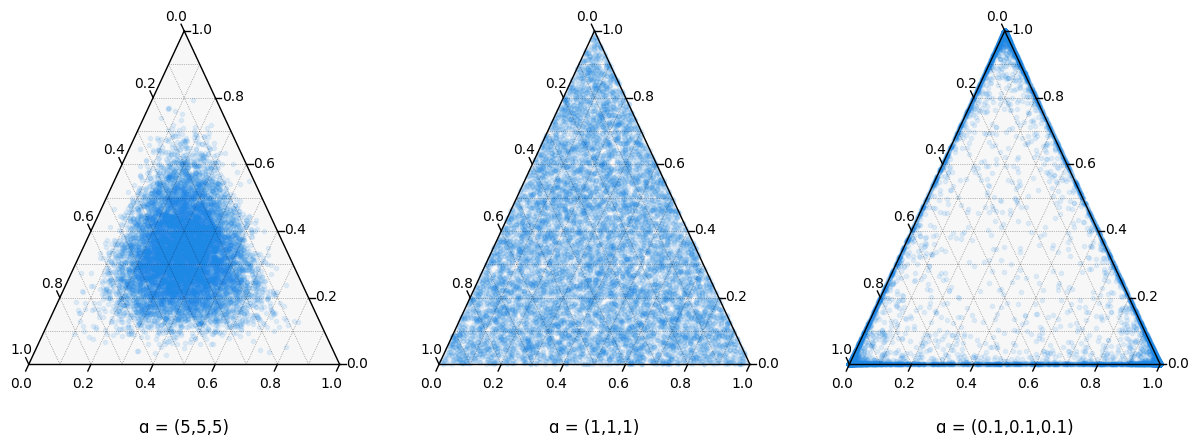
\includegraphics[width=1\textwidth]{resources/dirichlet_example.png}
    \caption{Scatter plots of 10000 samples of dirichlet distributions with different values of $\alpha$. For higher values, the distributions are more concentrated in the center. In the context of LDA, this means that each is assumed to have similar proportions of each topic for each document.}
    \label{fig:spelling_error_distribution}
\end{figure}


The number of topics $K$ is a parameter that is not related to the Dirichlet distributions. It is the number of topics that the model will try to identify.

The parameters $min\_df$ and $max\_df$ are used to filter out words that are too common or too rare, as such words may hurt the coherence of the model. For example, if a word occurs very frequently in a small number of documents, it could be attributed to a topic that it is not coherent to. Likewise for words that may occur rarely in a large number of documents. The values of these parameters completely depends on the corpus of documents.

\subsubsection*{Tuning the Parameters}

The parameters are not independant of each other. Every combination of the parameters yields a different coherence score, and the aim is to maximize this score. Two common approaches to parameter tuning are grid search and randomized search. 

Grid search is a brute force approach that tries every combination of parameters. The user specifies a range of values for each parameter and the algorithm tries every combination of these values. At the end, the combination of parameters that yields the highest coherence score is chosen. There are some problems with this approach. Firstly, it is computationally expensive. Producing an LDA model can take a long time. Calculating coherence scores for each set of parameters means that a module must produced using the parameters, and then the coherence score must be calculated. Depending on the parameter values, this can take a long time. For example, the first grid search that was performed for this project used a relatively conservative range of values for the parameters (around 7 values for each parameter), which resulted in 38000 models being produced, this took over 24 hours to complete. This means that the number of parameter values need to be limited in order to make the grid search feasible, which leads us to the second issue with this approach, which is that the best parameters may not be in the range of values that were specified. This means that the best parameters may not be found. Additionally, the grid search could cause overfitting, as the parameters are chosen based on the coherence score, which is calculated using the same data that the model was trained on.

The more feasible alternative to grid search is the randomized search. This approach is similar to grid search, but instead of trying every combination of parameters, it tries a random sample of the combinations for a set number of iterations. This allows for a larger range of values to be specified for the parameters, while keeping the task computationally feasible. In fact, the randomized search produced a higher range of coherence scores than the grid search, while taking less time to complete. 5000 models were evaluated in less than 4 hours, yielding a highest coherence score of over 0.38, while the grid search yielded the highest coherence score of 0.37. While this is not a significant difference, it makes evaluation a much cheaper and accessible task. Of course, the randomized search is not guaranteed to find the best parameters, but it is a good compromise between the grid search and the manual tuning of parameters.

\subsubsection{Limitations}

LDA is an unsupervised machine learning model that brings its own limitations with it. The most obvious limitation is that the model is not guaranteed to find the most accurate topics. While some $K_0$ number of topics may have a high coherence score, a different number of topics $K_1$ could also have a similar coherence score but with a different set of parameters. Though both models yield high coherence scores, it cannot be true that the corpus has both $K_0$ and $K_1$ topics. This problem arises from the metric that is used to evaluate the model. While the coherence metric has been shown to correlate with human interprability, it is still not a metric of human interpretability. This is a problem that is inherent to unsupervised machine learning models.

LDA is also a bag-of-words (BOW) model, so it does not account for the order of words in a document. This means that the model is not able to capture the context of words.

Another limitation is that LDA cannot capture correlations between topics. For example, if a corpus contains the topics "politics" and "tax", it is likely that there will be documents that contain both topics. However, Dirichlet distributions cannot capture this correlation.

Furthermore, like any other machine learning model, LDA is sensitive to the data that it's being fed. The model is only as good as the data that it gets. Noisy data will result in a noisy model. There is also the issue of having too little data. If the corpus is too small, the model might not be able to identify the topics. This requires some experimentation and there are no general guidelines as to what is considered to be a good sample size for the type of data that is being analyzed.